%% The openany option is here just to remove the blank pages before a new chapter
\documentclass[openany]{book}

\title{Manuel de Angular}

\usepackage{pagenote}
\usepackage[english,spanish]{babel}
\usepackage[utf8]{inputenc}
\usepackage{graphicx} 
\usepackage{hyperref,xcolor}
\usepackage{cite}
\usepackage{float}
\usepackage{pdfpages}
\usepackage{booktabs}
\usepackage{enumitem}
\usepackage{blindtext}
\usepackage{array}
\usepackage{array}
\usepackage{longtable}
\usepackage{setspace}
\usepackage{listings}

%%%%%%%%%%%%% For customising the endnote markers. Comment these out if you don't want them.
% To prefix each note number with the chapter number
\renewcommand{\thepagenote}{\thechapter-\arabic{pagenote}}

% To have a slightly different formatting for the endnote numbers in the text -- smaller text, sans-serif, square brackets
\renewcommand\notenumintext[1]{\space{\footnotesize\sffamily[FN-#1]}}

% To have a slightly different formatting for the endnote numbers in the notes section. Just the square brackets and sans-serif; normal size.
\renewcommand\notenuminnotes[1]{{\sffamily[FN-#1] }}

% If you want a different name/heading for the end notes
\renewcommand{\notesname}{End Notes}
\addto\captionsspanish{\renewcommand{\bibname}{Referencias}}
\renewcommand{\figurename}{Fig.}
\renewcommand{\bibname}{Referencias}

% Custom commands

\newcommand{\logo}[2]{\medskip\begin{center}\includegraphics[totalheight=2cm]{#1}\\\scriptsize\url{#2}\end{center}\bigskip}
\renewcommand\UrlFont{\color{black}\rmfamily\itshape}
\setlength{\parindent}{4em}
\setlength{\parskip}{1em}
\newcolumntype{M}[1]{>{\centering\arraybackslash}m{#1}}

% Custom margins

\setlength{\textwidth}{165mm}
\setlength{\textheight}{265mm}
\setlength{\topmargin}{-40mm}
\setlength{\oddsidemargin}{-1mm}
\setlength{\evensidemargin}{-1mm}

% Remove Chapter Headers

\makeatletter
\def\@makechapterhead#1{%
  \vspace*{50\p@}%
  {\parindent \z@ \raggedright \normalfont
    \interlinepenalty\@M
    \Huge \bfseries #1\par\nobreak
    \vskip 40\p@
  }}
\makeatother

% Remove indents

\setlength\parindent{0pt}

%%%%%%%%%%%%% End customisation


%% THIS LINE IS MANDATORY
\makepagenote

\begin{document}
 \begin{titlepage}

 \begin{center}\bf\sffamily
  
  \vspace*{10\baselineskip}
  {\Huge ANGULAR }\\
  \doublespacing
  {\LARGE Manual de uso.}\\
  \centering
  
\includegraphics{logos/angular.jpg}	\\
  {\large Realizado por}\\
  {\large Carmen María Soriano Tortosa}\\
  [1cm]
  {\large Módulo}\\
  {\large Desalloro Web en Entorno Cliente}  \\ 
\end{center}
\vfill
 \begin{flushright}
  {\bf\sffamily\large IES Celia Viñas, Almeria, 2019/2020 {\large }}
 \end{flushright}

\end{titlepage}

\tableofcontents % indice de contenidoss
\cleardoublepage

%Aqui se empieza a escribir el documento: 

\chapter{Introducción: ¿Qué es Angular?}

Angular es un framework de desarrollo para JavaScript creado por Google. La finalizar de este lengueje es facilitar el desarrollo de aplicaciones web SPA y además darnos herramientas para trabajar con los elementos de una web de una manera más sencilla e óptima. Además, permite separar de forma completa el front-end y el back-end de la aplicación. 

Las aplicaciones creadas en Angular pueden ser usadas en dispositivos móviles y de escritorio gracias a que es un framework cross-platform, usando el nodelo vista controlador (MVC) y la ejecución es llevada por el lado del cliente, provocando así que todo dependa en gran parte del navegador.  

\section{¿Que es una aplicación SPA?}
Una web SPA(Single Page App) es una aplicación web de una sóla página, en la cual la navegación entre secciones y páginas de la aplicación, así como la carga de datos, se realiza de manera dinámica, casi instantánea, asincronamente haciendo llamadas al servidor, y sobretodo sin resgrescar la página en ningún momento. 

Las aplicaciones que podemos hacer con Angular son reactivas y no recargan el navegador, todo es muy dinámico y asincrono con ajax. 

\section{La historia de Angular}
AngularJS comenzó a ser desarrollado eb 2009 por Misko Hevey, siendo al principio un servicio de lmacenamiento online para archivos JSON donde el precio dependia del peso de cada archivo. Tiempo después abandonó el proyecto y se lanzó angular como un proyecto open-source.

La primera versión de Angular, conocida realmente como AngularJS o Angular 1 fue lanzado en 2010, después en 2014 fue lanzada Angular2, en un principio se pensó que seria una nueva versión, pero en realidad son framework completa diferente, teniendo cada uno sus ventajas. 

En 2016 se lazó la primera versión estble de Angular2, conocida popularmente como Angular. 

\section{Características de Angular}
\begin{itemize}
\item \textbf{Desarrollo Móvil:} El desarrollo de aplicaciones de escritorio es mucho más fácil cuando primero se manejan los problemas de rendimiento en el desarrollo móvil.
\item \textbf{Modularidad:} Para desarrollar una nueva funcionalidad esta se empaqueta en un módulo, produciendo un núcleo más ligero y más rápido.
\item \textbf{Compatibilidad:} Es compatible con los navegadores más modernos y recientes.
\end{itemize}

\chapter{Instalación de Angular }
Para poder usar Angular necesitaremos tener instalado NodeJS4, NPM3 o superior (que se instala en conjunto con NodeJS), y como recomandación, pero no obligación, GitHub y un editor de texto como puede ser Visual Estudio Code. 
\\ \textbf{PASOS DE INSTALACIÓN}\\
\textbf{1. Instalamos NodeJS y rpm}\\
\textbf{2.Creamos una carpera con el nombre que deseemos, en mi caso a sido Proyecto\\ 3.Dentro de esa carpeta generamos los siguientes archivos:}
\begin{itemize}
  \item \textbf{package.json:} Identifica las dependencias de paquetes npm para el proyecto.
  \begin{lstlisting}
    {
    "name": "angular-quickstart",
    "version": "1.0.0",
    "scripts": {
      "start": "tsc && concurrently \"tsc -w\" \"lite-server\" ",
      "lite": "lite-server",
      "tsc": "tsc",
      "tsc:w": "tsc -w"
    },
    "licenses": [
      {
        "type": "MIT",
        "url": "https://github.com/angular/angular.io/blob/master/LICENSE"
      }
    ],
    "dependencies": {
      "@angular/common": "~2.2.0",
      "@angular/compiler": "~2.2.0",
      "@angular/core": "~2.2.0",
      "@angular/forms": "~2.2.0",
      "@angular/http": "~2.2.0",
      "@angular/platform-browser": "~2.2.0",
      "@angular/platform-browser-dynamic": "~2.2.0",
      "@angular/router": "~3.2.0",
      "@angular/upgrade": "~2.2.0",
      "angular-in-memory-web-api": "~0.1.15",
      "core-js": "^2.4.1",
      "reflect-metadata": "^0.1.8",
      "rxjs": "5.0.0-beta.12",
      "systemjs": "0.19.39",
      "zone.js": "^0.6.25"
    },
    "devDependencies": {
      "@types/core-js": "^0.9.34",
      "@types/node": "^6.0.45",
      "concurrently": "^3.0.0",
      "lite-server": "^2.2.2",
      "typescript": "^2.0.3"
    }
  }
  \end{lstlisting}
  \vspace*{5\baselineskip}
  \item \textbf{tsconfig.json:} Define la configuración de TypeScript y como compilara los archivos JavaScript.
  \begin{lstlisting}
    {
  "compilerOptions": {
    "target": "es5",
    "module": "commonjs",
    "moduleResolution": "node",
    "sourceMap": true,
    "emitDecoratorMetadata": true,
    "experimentalDecorators": true,
    "removeComments": false,
    "noImplicitAny": false
  }
}
\end{lstlisting}
  \item \textbf{Systemjs.config.js:} Proporcionará la configuración de cómo serán cargados los módulos del proyecto.
  \begin{lstlisting}
    /**
 * System configuration for Angular samples
 * Adjust as necessary for your application needs.
 */
(function (global) {
  System.config({
    paths: {
      // paths serve as alias
      'npm:': 'node_modules/'
    },
    // map tells the System loader where to look for things
    map: {
      // our app is within the app folder
      app: 'app',
      // angular bundles
      '@angular/core': 'npm:@angular/core/bundles/core.umd.js',
      '@angular/common': 'npm:@angular/common/bundles/common.umd.js',
      '@angular/compiler': 'npm:@angular/compiler/bundles/compiler.umd.js',
      '@angular/platform-browser': 'npm:@angular/platform-browser/bundles/platform-browser.umd.js',
      '@angular/platform-browser-dynamic': 'npm:@angular/platform-browser-dynamic/bundles/platform-browser-dynamic.umd.js',
      '@angular/http': 'npm:@angular/http/bundles/http.umd.js',
      '@angular/router': 'npm:@angular/router/bundles/router.umd.js',
      '@angular/forms': 'npm:@angular/forms/bundles/forms.umd.js',
      '@angular/upgrade': 'npm:@angular/upgrade/bundles/upgrade.umd.js',
      // other libraries
      'rxjs':                      'npm:rxjs',
      'angular-in-memory-web-api': 'npm:angular-in-memory-web-api/bundles/in-memory-web-api.umd.js'
    },
    // packages tells the System loader how to load when no filename and/or no extension
    packages: {
      app: {
        main: './main.js',
        defaultExtension: 'js'
      },
      rxjs: {
        defaultExtension: 'js'
      }
    }
  });
  })(this);
  \end{lstlisting}
  \vspace*{5\baselineskip}
\end{itemize}
\textbf{4. Creación de reporitorio en Git} Este paso es opcional.
\\ Para crear el repositorio en Git, a través de nuestro CMD navegamos hasta la carpeta contenedora de los archivos que creamos anteriormente y procedemos a seguir los siguientes pasos: 
\begin{itemize}
  \item Comprobamos que tenemos instaldo NodeJS, NPM y Git (node -v, npm -v y git --version)
  \\ 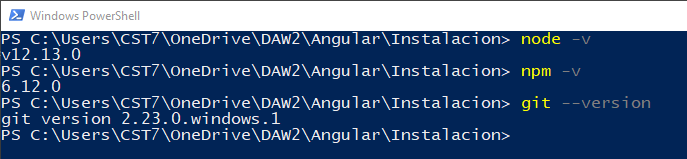
\includegraphics{logos/comandos.png}\\
  \item Iniciamos un reporitorio git con el comando git init.
  \item Agregamos nuestros archivos iniciales al repositorio con el comando git add. (Recuerda ponerle el punto al final)
  \item Hacemos el comit inicial con el comando git commit -m "Comentario"
  \\ 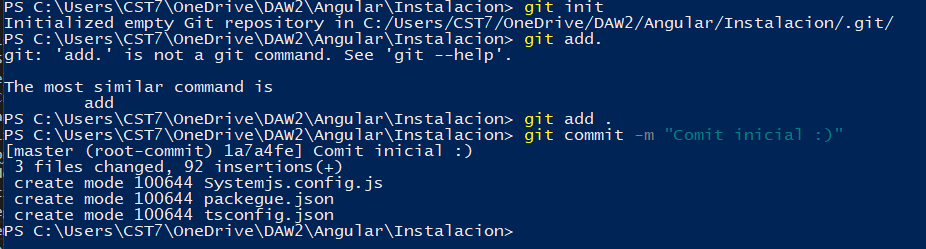
\includegraphics{logos/comandos2.png}
\end{itemize}
\textbf{5. Instalamos los paquetes necesarios: }

Para instalar los paquetes necesarios usaremos el comando npm install, tras usar este comando se nos generara una carpeta llamada node\_modules dentro de nuestra carpeta. También creamos una carpeta App por lo que nuestra carpeta quedará de la siguiente manera:

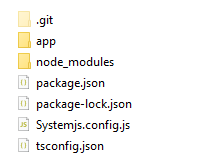
\includegraphics{logos/carpeta.png}

\pagebreak
\vspace*{5\baselineskip}
\textbf{6. Componentes:}

Dentro de la carpera App, creamos un archivo llamado \textbf{app.component.ts} con el siguiente contenido: 
\begin{lstlisting}
  import { Component } from '@angular/core';
  @Component({
    selector: 'my-app',
    template: '<h1>Hello Angular!</h1>'
  })
  export class AppComponent { }
\end{lstlisting}

\textbf{7. Módulo inicial:}

Dentro de un proyecto de Angular necesateremos siempre al menos un módulo, este se encontrará dentro de la carpeta App, y lo crearemos con el nombre \textbf{app.module.ts} y con el siguiente contenido:
\begin{lstlisting}
  import { NgModule }      from '@angular/core';
  import { BrowserModule } from '@angular/platform-browser';
  import { AppComponent }   from './app.component';
  @NgModule({
    imports:      [ BrowserModule ],
    declarations: [ AppComponent ],
    bootstrap:    [ AppComponent ]
  })
  export class AppModule { }
\end{lstlisting}

\textbf{8. Main: }

Ahora crearemos nevamente dentro de la carpeta App un archivo llamado \textbf{main.ts} con el siguiente conrenido: 
\begin{lstlisting}
  import { platformBrowserDynamic } from '@angular/platform-browser-dynamic';
  import { AppModule } from './app.module';
  const platform = platformBrowserDynamic();
  platform.bootstrapModule(AppModule);
\end{lstlisting}

\textbf{9. Index.html}

Ahora dentro de nuestra carptera principal, en mi caso llamada Proyecto, y creamos un archivo llamado \textbf{index.html} que contenga el siguiente código: (¡Cuidado el código sigue en la siguiente página!)
\begin{lstlisting}
  <html>
  <head>
    <title>Angular QuickStart</title>
    <meta charset="UTF-8">
    <meta name="viewport" content="width=device-width, initial-scale=1">
    <!-- 1. Load libraries -->
     <!-- Polyfill for older browsers -->
    <script src="node_modules/core-js/client/shim.min.js"></script>
    <script src="node_modules/zone.js/dist/zone.js"></script>
    <script src="node_modules/reflect-metadata/Reflect.js"></script>
    <script src="node_modules/systemjs/dist/system.src.js"></script>
    <!-- 2. Configure SystemJS -->
    <script src="systemjs.config.js"></script>
    <script>
      System.import('app').catch(function(err){ console.error(err); });
    </script>
  </head>
\end{lstlisting}
  \pagebreak 
  \vspace*{5\baselineskip}
  \begin{lstlisting}
  <!-- 3. Display the application -->
  <body>
    <my-app>Loading...</my-app>
  </body>
</html>
\end{lstlisting}

\textbf{9. Ejecución: }

Para ejecutar nuestro proyecto usaremos el comando npm start. Al ejecutar este comando se nos crearan los siguientes archivos:
\begin{center}
  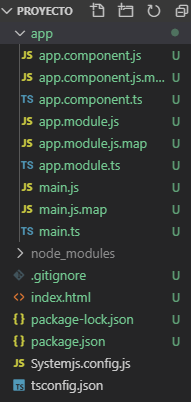
\includegraphics{logos/contenido_carpeta.png}
\end{center}
Al ejecutarlo se nos abrirá una pestaña del navegador con la dirección localhost con el mensaje ¡Hola Angular!









\addcontentsline{toc}{chapter}{9. Referencias}
\begin{thebibliography}{References}
\bibitem{1} \textsc{¿Cuántas horas es aconsejable dormir según nuestra edad?} [\url{http://www.abc.es/familia-vida-sana/20150212/abci-dormir-horas-201502121131.html}]
\bibitem{2} \textsc{JavaScript} [\url{https://es.wikipedia.org/wiki/JavaScript}]
\bibitem{3} \textsc{TypeScript} [\url{https://es.wikipedia.org/wiki/TypeScript}]
\bibitem{4} \textsc{Node.js} [\url{https://es.wikipedia.org/wiki/Node.js}]
\bibitem{5} \textsc{Express.js} [\url{https://en.wikipedia.org/wiki/Express.js}]
\bibitem{6} \textsc{Angular2} [\url{https://www.tutorialspoint.com/angular2/}]
\bibitem{7} \textsc{Firebase} [\url{https://en.wikipedia.org/wiki/Firebase}]ZFZXC
\bibitem{8} \textsc{Firebase (Github)} [\url{https://github.com/firebase/}]
\bibitem{9} \textsc{Selenium} [\url{ttps://es.wikipedia.org/wiki/Selenium}]
\bibitem{10} \textsc{Jasmine} [\url{ttps://en.wikipedia.org/wiki/Jasmine_(JavaScript_testing_framework)}]
\bibitem{11} \textsc{Protractor} [\url{https://www.adictosaltrabajo.com/tutoriales/introduccion-a-protractor/}]
\bibitem{12} \textsc{Visual Studio Code} [\url{ttps://en.wikipedia.org/wiki/Visual_Studio_Code}]
\bibitem{13} \textsc{Scrum: The Art of Doing Twice the Work in Half the Time} [Autor: Jeff Sutherland]
\bibitem{14} \textsc{UML Distilled} [Autor: Martin Fowler]
\bibitem{15} \textsc{Travis} [\url{https://en.wikipedia.org/wiki/Travis_CI}]
\bibitem{16} \textsc{Sprint} [\url{https://proyectosagiles.org/ejecucion-iteracion-sprint/}]
\bibitem{17} \textsc{¿Cada cuánto solemos renovar el móvil en España?} [\url{http://byemovil.com/renovar-el-movil}]
\bibitem{18} \textsc{Understanding Model-View-Controller} [Autor: Stefano Borini \url{https://www.gitbook.com/book/stefanoborini/modelviewcontroller/details}]

\end{thebibliography}

\end{document}